\documentclass[a4paper,11pt]{article}

\usepackage[T1]{fontenc}
\usepackage[polish]{babel}
\usepackage[utf8]{inputenc}
\usepackage{lmodern}
\selectlanguage{polish}
\usepackage[top=2cm, bottom=2cm, left=3cm, right=3cm]{geometry}

\makeatletter
\newcommand{\linia}{\rule{\linewidth}{0.4mm}}
\renewcommand{\maketitle}{\begin{titlepage}
    \vspace*{2cm}
    \begin{center}\LARGE
    Politechnika Warszawska\\
    Wydział Elektryczny\\
    \end{center}
    \vspace{5cm}
    \noindent\linia
    \begin{center}
      \LARGE \textsc{\@title}
         \end{center}
     \linia
    \vspace{0.5cm}
    \begin{flushright}
    \begin{minipage}{5cm}
    \textit{Autorzy:}\\
    \normalsize \textsc{\@author} \par
    \end{minipage}
    \vspace{5cm}
     \end{flushright}
    \vspace*{\stretch{6}}
    \begin{center}
    \@date
    \end{center}
  \end{titlepage}%
}
\makeatother
\author{Grzegorz Kopyt\\
Daniel Sporysz}
\title{Specyfikacja Implementacyjna \\
"WireWorld"}

\usepackage{graphicx}
\begin{document}

\maketitle


\tableofcontents
\vspace{1cm}
\noindent\linia





\section{Diagram klas}


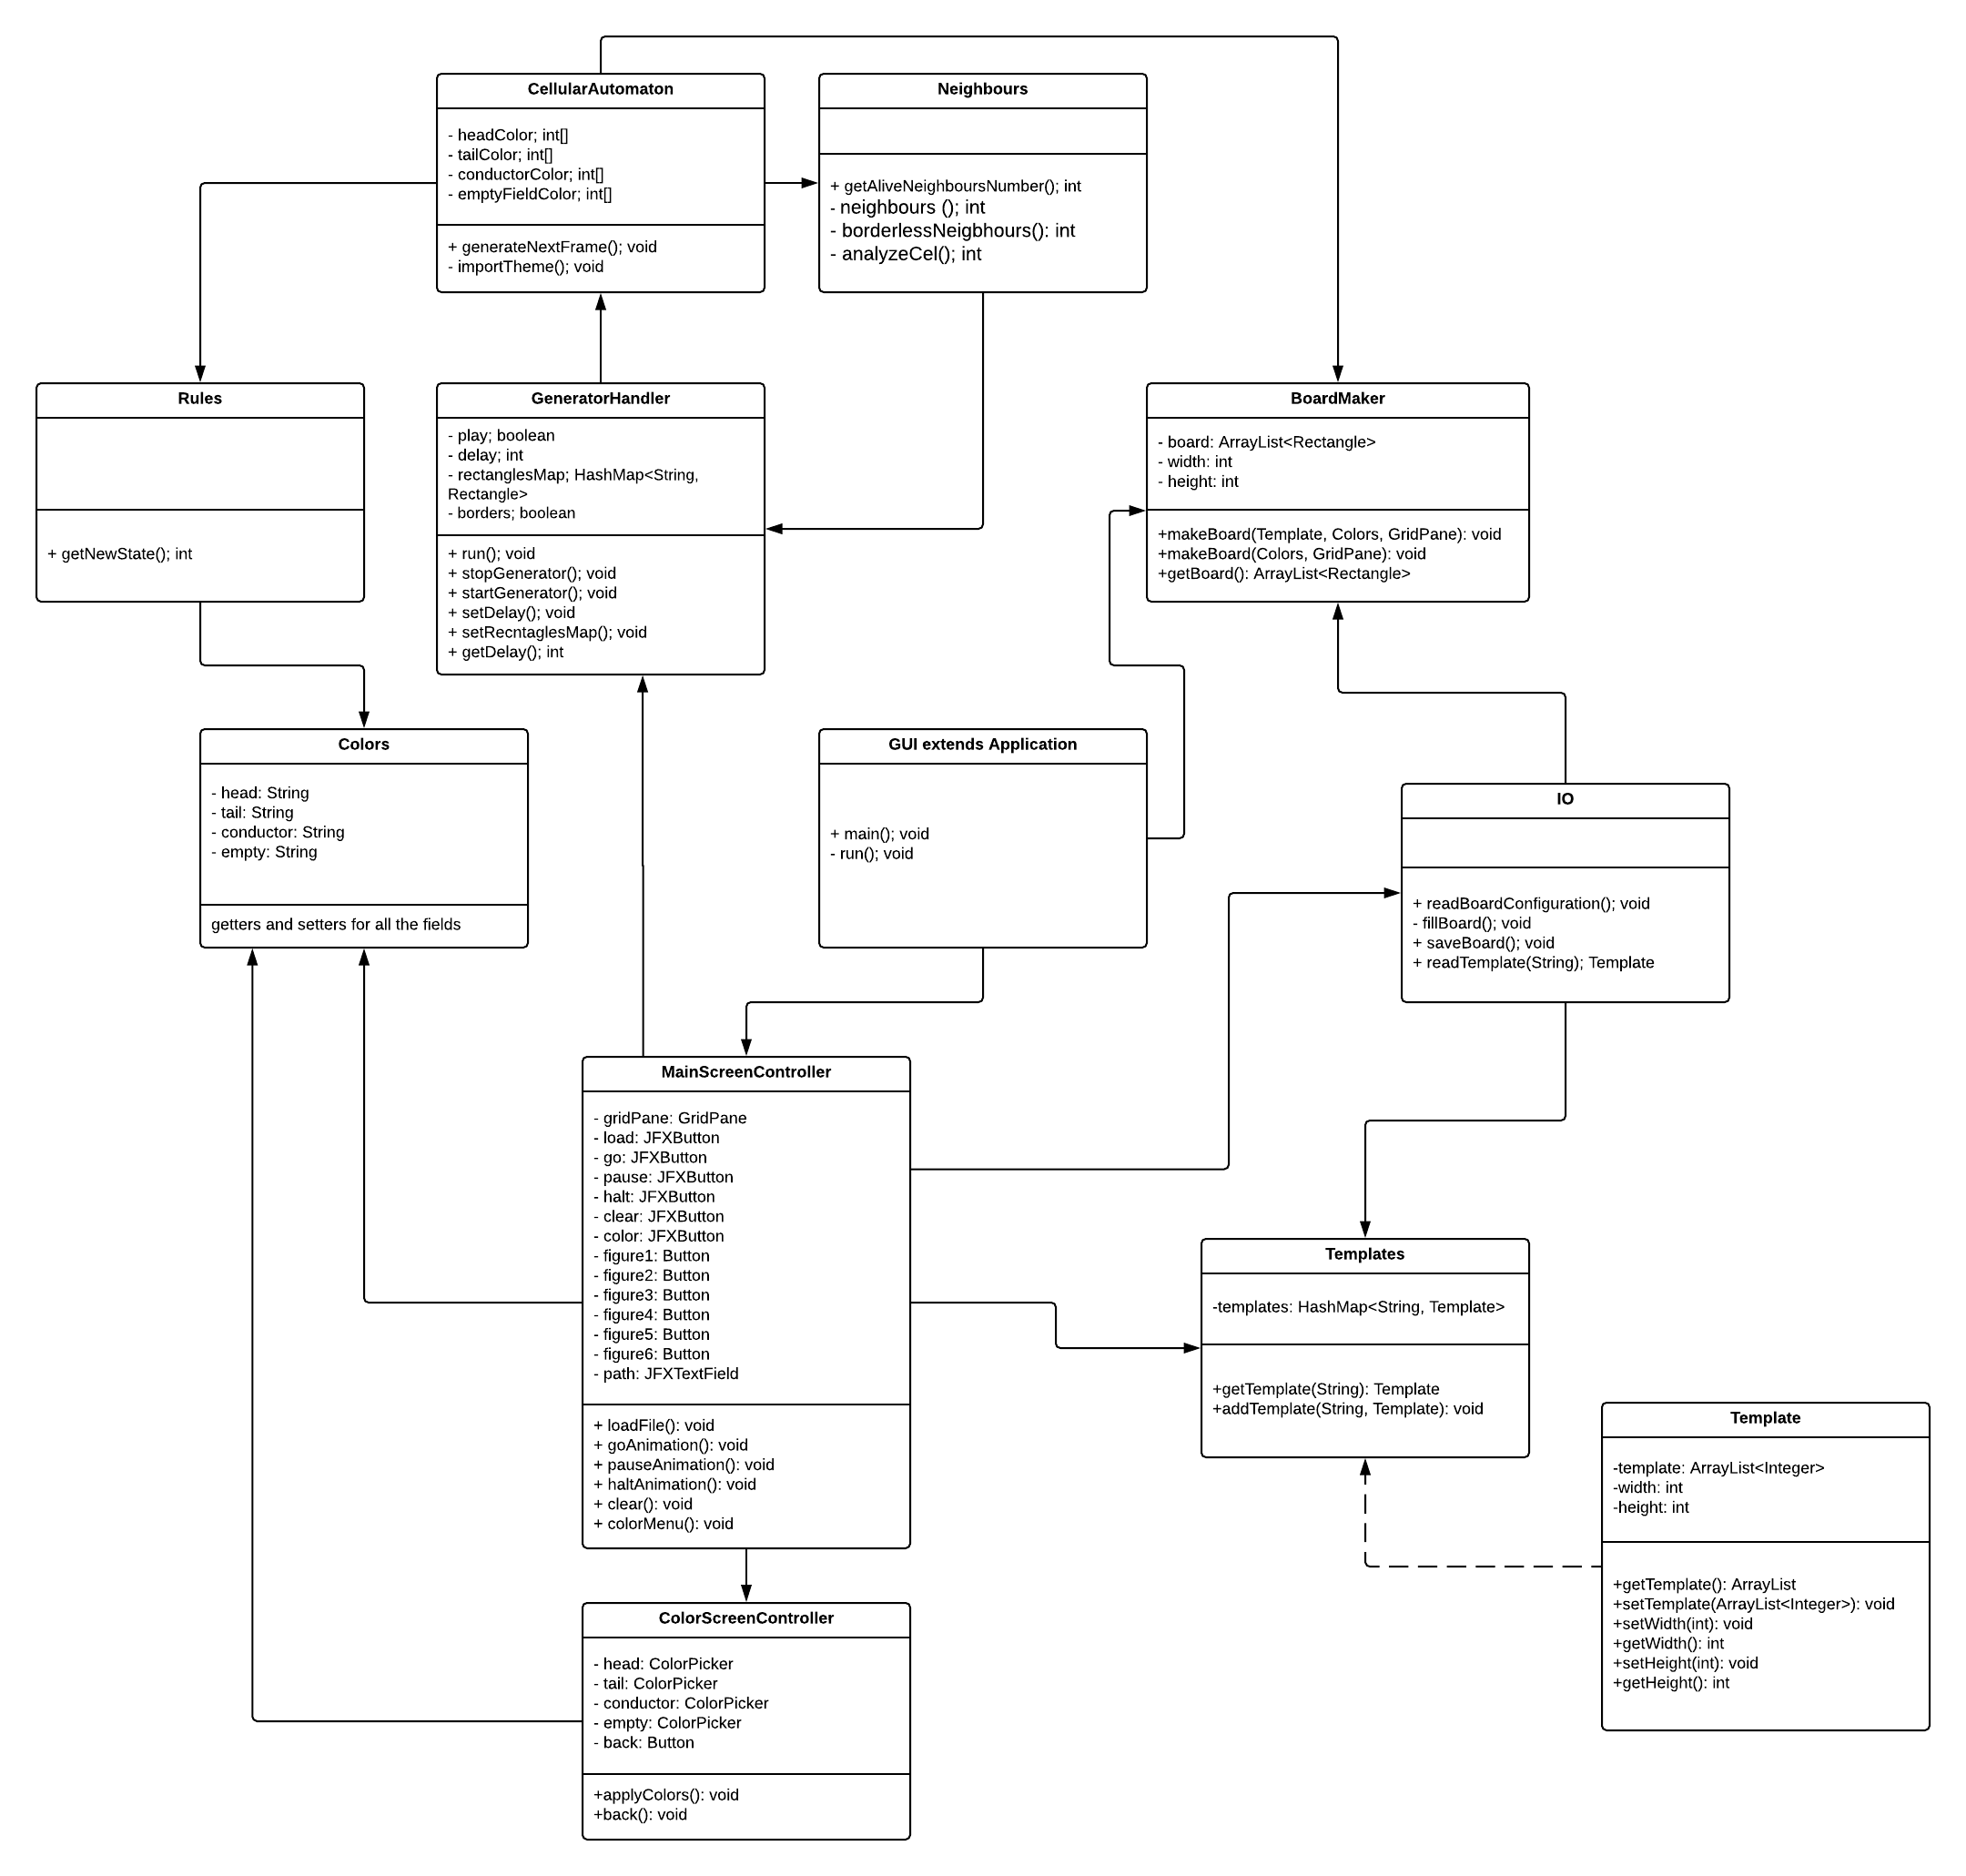
\includegraphics[width=\textwidth]{DiagramKlas}

\noindent\linia


\section{Diagram pakietów}
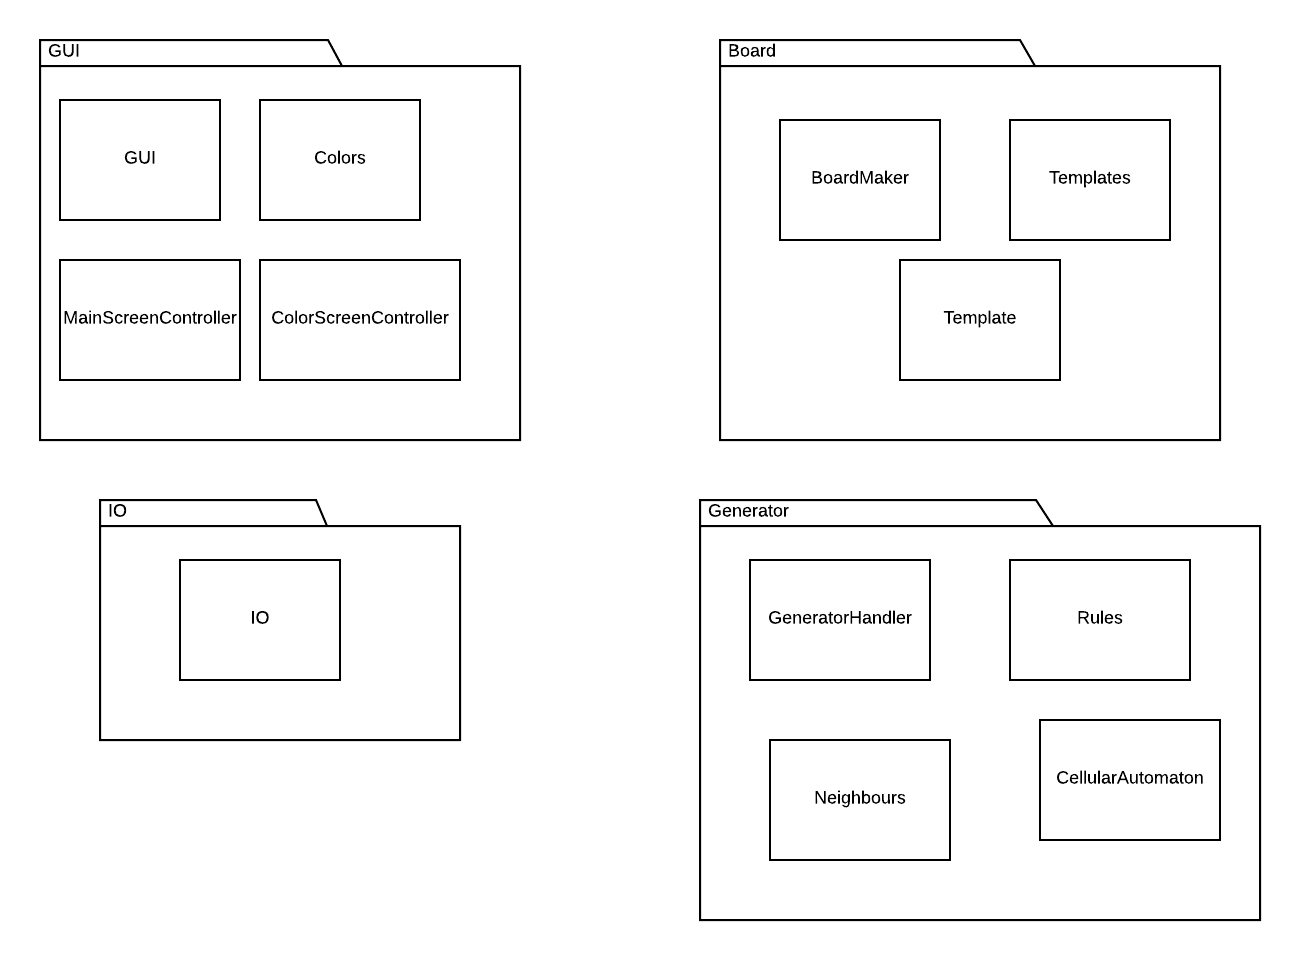
\includegraphics[width=\textwidth]{DiagramPakiet}







\noindent\linia
\section{Pakiet GUI}

Wykonany przy pomocy technologii javafx, zawiera dodatkową bibliotekę: jfoenix.

\subsection{Pliki .fxml:}
\begin{itemize}
\item MainScreen.fxml
\item ColorScreen.fxml
\end{itemize}

\subsection{GUI}
Rozszerza klasę Application z javafx.
\subsubsection{Pola}
brak
\subsubsection{Metody}
\begin{itemize}
\item \textbf{main}

Standardowo wywołuje metodę launch.
\item \textbf{start}

Wczytuje plik MainScreen.fxml, przygotowuje całą scenę i wyświetla ją w wymiarach (800, 600).
\end{itemize}


\subsection{MainScreenController}
Kontroler sceny MainScreen.fxml.
\subsubsection{Pola}
\begin{itemize}
\item GridPane \textit{gridPane}
\item JFXButton \textit{load}
\item JFXButton \textit{go}
\item JFXButton \textit{pause}
\item JFXButton \textit{halt}
\item JFXButton \textit{clear}
\item JFXButton \textit{color}
\item Button \textit{figure1}
\item Button \textit{figure2}
\item Button \textit{figure3}
\item Button \textit{figure4}
\item Button \textit{figure5}
\item Button \textit{figure6}
\item JFXTextField \textit{path}
\end{itemize}
\subsubsection{Metody}
\begin{itemize}
\item void \textbf{loadFile()}

Standardowo wywołuje metodę launch.
\item void \textbf{goAnimation()}

Uruchamia animacje wywołując metodę z klasy Animation.
\item void \textbf{pauseAnimation()}

Pauzuje animacje metodą z klasy Animation.
\item void \textbf{haltAnimation()}

Powoduje powrót animacji do punktu początkowego.
\item void \textbf{clear()}

Zmienia kolor każdej komórki w tablicy na biały.
\item void \textbf{colorMenu()}

Wyświetla okno z pliku ColorMenu.fxml
\end{itemize}





\subsection{ColorScreenController}
Kontroler sceny ColorScreen.fxml.
\subsubsection{Pola}
\begin{itemize}
\item ColorPicker \textit{head}
\item ColorPicker \textit{tail}
\item ColorPicker \textit{conductor}
\item ColorPicker \textit{empty}

\end{itemize}
\subsubsection{Metody}
\begin{itemize}
\item void \textbf{back()}

Powoduje powrót do MainScreen.
\item void \textbf{applyColors()}

Pobiera z obiektów klasy ColorPicker informacje o kolorach i przekazuje je klasie Colors.

\end{itemize}
\noindent\linia




\subsection{Colors}
Kontroler sceny ColorScreen.fxml.
\subsubsection{Pola}
\begin{itemize}
\item String head
\item String tail
\item String conductor
\item String empty

\end{itemize}
\subsubsection{Metody}
\begin{itemize}
\item String \textbf{getHead()}
\item void \textbf{setHead()}
\item String \textbf{getTail()}
\item void \textbf{setTail()}
\item String \textbf{getConductor()}
\item void \textbf{setConductor()}
\item String \textbf{getEmpty()}
\item void \textbf{setEmpty()}
\subsubsection{Konstruktor}
Domyślne kolory to:
\begin{itemize}
\item head - żółty
\item tail - czerwony
\item conductor - czarny
\item empty - biały
\end{itemize}
\end{itemize}
\noindent\linia







\section{Pakiet IO}
\subsection{IO}
krótki opis klasy
\subsubsection{Pola}

\subsubsection{Metody}



\noindent\linia

\section{Pakiet Board}

\subsection{BoardMaker}
Odpowiada za stworzenie tablicy obiektów klasy Rectangle (\textit{board}). Tablica ta będzie służyła jako obszar edytowany przez użytkownika, a także będzie na niej wyświetlana animacja.
\subsubsection{Pola}
\begin{itemize}
\item ArrayList<Rectangle> \textit{board}
\item int \textit{width}
\item int \textit{height}
\end{itemize}
\subsubsection{Metody}
\begin{itemize}
\item void \textbf{makeBoard(Template, Colors, GridPane)}

Metoda tworzy tablicę \textit{board} obiektów klasy Rectangle na podstawie wzoru podanego w Template o 30 kwadratach w rzędzie i 30 kwadratach w kolumnie.
Wymiary obiektów Rectangle wynoszą (20, 20).
Wszystkie obiekty dodane zostają do kolekcji \textit{board}.
Obiektom zostaje nadane ID jako kolejne liczby naturalne całkowite zaczynając od 1.
Kolor wypełnienia obiektów nadawany jest zgodnie z zawartością Colors, obramowanie - czarne.
Tablica tworzona jest poprzez dodanie obiektów do  GridPane.
Docelowy GridPane znajduje się w klasie MainScreenController.
\item void \textbf{makeBoard(Colors, GridPane)}

Metoda tworzy tablicę \textit{board} obiektów klasy Rectangle o 30 kwadratach w rzędzie i 30 kwadratach w kolumnie.
Wymiary obiektów Rectangle wynoszą (20, 20).
Wszystkie obiekty dodane zostają do kolekcji \textit{board}.
Obiektom zostaje nadane ID jako kolejne liczby naturalne całkowite zaczynając od 1.
Kolor wypełnienia obiektów nadawany jest zgodnie z zawartością Colors, obramowanie - czarne.
Tablica tworzona jest poprzez dodanie obiektów do  GridPane.
Docelowy GridPane znajduje się w klasie MainScreenController.

\item ArrayList<Rectangle> \textbf{getBoard()}
\end{itemize}



\subsection{Template}
Klasa reprezentująca wzór obiektu do wstawiania na tablice \textit{board}. Wzór przechowywany jest w tablicy \textit{template} jako ciąg liczb 0(pusty), 1(przewodnik), 2(ogon), 3(głowa). Przy tworzeniu wzorów należy uwzględnić to, że rozmiar tablicy wynosi 30 kwadratów na 30 kwadratów. 
\subsubsection{Pola}
\begin{itemize}
\item ArrayList<Integer> \textit{template}
\item int \textit{width}
\item int \textit{height}
\end{itemize}

\subsubsection{Metody}
\begin{itemize}
\item Template \textbf{getTemplate()}
\item void \textbf{setTemplate(ArrayList<Integer>)}
\item void \textbf{setWidth(int)}
\item int \textbf{getWidth()}
\item void \textbf{setHeight(int)}
\item int \textbf{getHeight()}
\end{itemize}


\subsection{Templates}
Przeznaczeniem klasy jest przechowywanie obiektów klasy template w kolekcji.
\subsubsection{Pola}
\begin{itemize}
\item HashMap<String, Template> \textit{templates}
\end{itemize}
\subsubsection{Metody}
\begin{itemize}
\item Template \textbf{getTemplate(String)}

Metoda otrzymawszy klucz klasy \textit{String} zwraca obiekt klasy Template z kolekcji \textit{templates}.
\item void \textbf{addTemplate(String, Template)}

Metoda dodaje do kolekcji \textit{templates} obiekt klasy Template i nadaje mu klucz podany jako zmienna klasy String.
\end{itemize}
\noindent\linia

\section{Pakiet Generation}



\subsection{GenerationsHandler}
krótki opis klasy
\subsubsection{Pola}
\begin{itemize}
\item typ  \textit{nazwa}
\end{itemize}
\subsubsection{Metody}
\begin{itemize}
\item typ  \textbf{nazwa}

opis metody
\end{itemize}






\subsection{CellularAutomaton}
krótki opis klasy
\subsubsection{Pola}
\begin{itemize}
\item typ  \textit{nazwa}
\end{itemize}
\subsubsection{Metody}
\begin{itemize}
\item typ  \textbf{nazwa}

opis metody
\end{itemize}




\subsection{Rules}
krótki opis klasy
\subsubsection{Pola}
\begin{itemize}
\item typ  \textit{nazwa}
\end{itemize}
\subsubsection{Metody}
\begin{itemize}
\item typ  \textbf{nazwa}

opis metody
\end{itemize}


\noindent\linia
\section{Przepływ Sterowania}




\noindent\linia
\section{Testy klas}

\subsection{GUI}
\subsubsection{MainScreenController}
\begin{description}

\item[Scenariusze] \hfill
\begin{enumerate}
\item
\item 
\item
\item
\item 
\end{enumerate}

\item[Kryteria oceny poprawnej pracy] \hfill
\begin{enumerate}
\item 
\item
\item
\item 
\item 
\end{enumerate}

\end{description}

\subsection{IO}
\subsubsection{IO}
\begin{description}

\item[Scenariusze] \hfill
\begin{enumerate}
\item
\item 
\item
\item
\item 
\end{enumerate}

\item[Kryteria oceny poprawnej pracy] \hfill
\begin{enumerate}
\item 
\item
\item
\item 
\item 
\end{enumerate}

\end{description}

\subsection{Board}
\subsubsection{BoardMaker}
\begin{description}

\item[Scenariusze] \hfill
\begin{enumerate}
\item
\item 
\item
\item
\item 
\end{enumerate}

\item[Kryteria oceny poprawnej pracy] \hfill
\begin{enumerate}
\item 
\item
\item
\item 
\item 
\end{enumerate}

\end{description}

\subsection{Generation}
\subsubsection{GenerationsHandler}
\begin{description}

\item[Scenariusze] \hfill
\begin{enumerate}
\item
\item 
\item
\item
\item 
\end{enumerate}

\item[Kryteria oceny poprawnej pracy] \hfill
\begin{enumerate}
\item 
\item
\item
\item 
\item 
\end{enumerate}

\end{description}


\end{document}



